\chapter{Conservación de la energía.}
\section{Definiciones.}
\begin{itemize}
	\item Presión de remanso:
	\[P_0=P+\rho\dfrac{v^2}{2}\]
	\item Entalpía de remanso:
	\[P_0+U=cte\]
	\item Bernouille:
	\[h_0=h+\dfrac{v^2}{2}\rightarrow h= e +\dfrac{P}{\rho}\]
	
	Donde $e$ es la energía interna.
\end{itemize}
\section{Conservación de la energía en forma integral.}
Se elige como volumen de control aquel que queda encerrado por la entrada, la salida, la pared del conducto y las posibles máquinas rotativas que pudiese haber.
\begin{figure}[H]
	\centering
		\begin{circuitikz}
			\tikzstyle{every node}=[font=\LARGE]
			\draw [ color={rgb,255:red,255; green,0; blue,0} , dashed] (1.5,12.5) rectangle  (11.5,8.5);
			\draw [ color={rgb,255:red,255; green,0; blue,0} , dashed] (6,10.5) circle (1.5cm);
			\draw [short] (1.25,12.75) -- (11.75,12.75);
			\draw [short] (1.25,8.25) -- (11.75,8.25);
			\draw  (6,10.5) circle (1.4cm) node {\normalsize Maquina rotativa} ;
			\node [font=\normalsize, color={rgb,255:red,255; green,0; blue,0}] at (11,12) {$V_c$};
			\node [font=\normalsize] at (1,10.5) {$S_e$};
			\node [font=\normalsize] at (11.75,10.25) {$S_s$};
			\node [font=\normalsize] at (7.75,10.5) {$S_m$};
			\node [font=\normalsize] at (6.75,13) {$S_p$};
		\end{circuitikz}
		\caption{Diagrama genérico de un posible conducto.}
	\label{fig:my_label}
\end{figure}

\section{Bombas/compresores y turbinas.}
\begin{itemize}
	\item Cuando se trabaja con gases el trabajo ideal desarrollado por un compresor es:
	\[\dot{W}_C=G(h_{0_s}-h_{0_e})\]
	
	Donde $G$ es el gasto y por conservación de la masa se puede expresar en magnitud de entrada o de salida.
	\[G=\rho_e A_e v_e=\rho_s A_s v_s\]
	
	\item Cuando se trabaja con líquidos el trabajo ideal desarrollado por una bomba es:
	\[\dot{W}=Q(P_{0_s}-P_{0_e})\]
\end{itemize}

El criterio de signos del trabajo es:
\begin{itemize}
	\item $\dot{W}>0$ para bombas y compresores.
	\item $\dot{W}<0$ para turbinas.
\end{itemize}


Si se trabaja con máquinas reales, cuando se habla del trabajo real, se refiere al trabajo que sería necesario aportar o que se recibiría de la máquina teniendo en cuenta su rendimiento. Por ello:
\begin{itemize}
	\item $\dot{W}_{B_{Real}}=\dfrac{\dot{W}_{B_{ideal}}}{\eta_B}$, se debe aportar más energía para realizar el trabajo útil.
	\item $\dot{W}_{C_{Real}}=\dfrac{\dot{W}_{C_{ideal}}}{\eta_C}$, se debe aportar más energía para realizar el trabajo útil.
	\item $\dot{W}_{T_{Real}}=\dot{W}_{T_{ideal}}\cdot \eta_T$, el trabajo obtenido a través de la turbina es menor debido a las pérdidas.
\end{itemize}
\section{Pérdidas de carga.}
Cuando el fluido pasa por codos, descarga a conducto o ensancha de forma brusca se producen pérdidas en la presión de remanso. Para modelarlo, se emplea un factor $K_P$ de pérdidas.
\section{Factor de fricción (f).}
sd
\section{Diagrama de Moody.}
\begin{figure}[H]
	\centering
	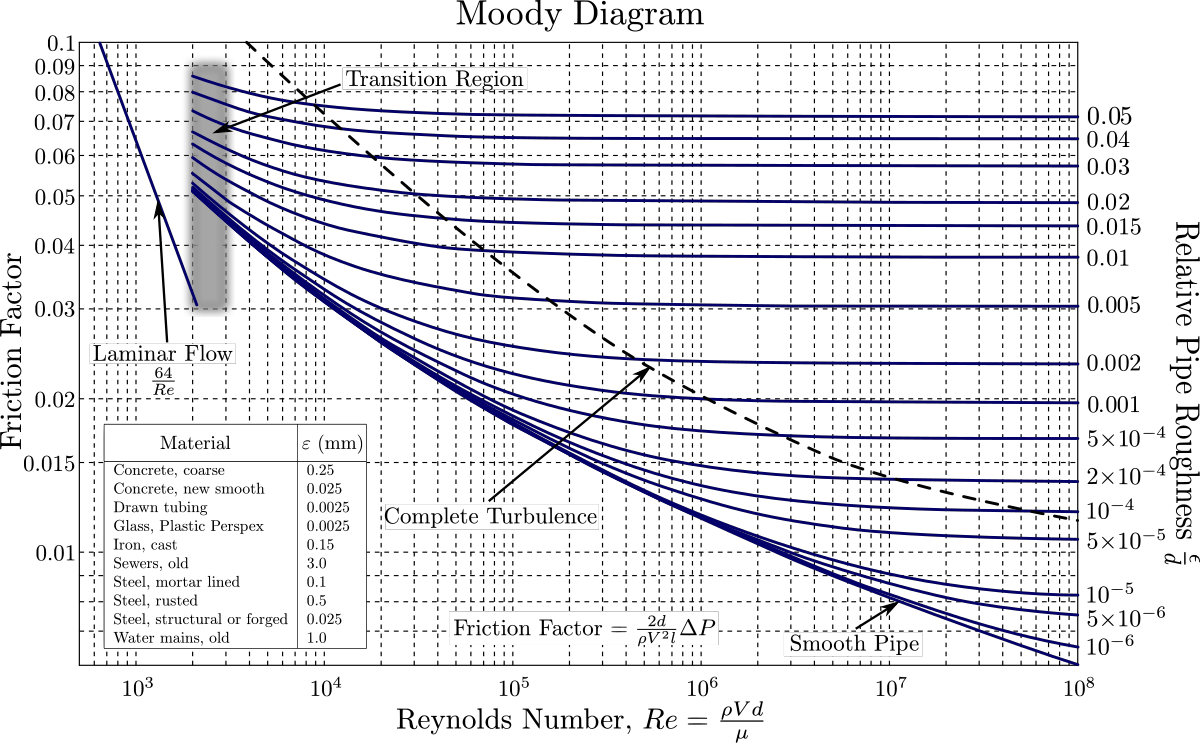
\includegraphics[width=1\linewidth]{ImagenesTema6/Moody}
	\caption{Diagrama de Moody.}
	\label{fig:moody}
\end{figure}
